\chapter{Building and Running the Monitoring Application}
\lhead{\emph{Appendix B - Building and Running the Monitoring Application}}  

\section{Prerequisites} 

The Monitoring Application has the following prerequisites:

\begin{enumerate}
	
	\item Java Development Kit V8, available from \newline https://www.oracle.com/technetwork/java/javaee/downloads.
	\item Maven 3.x, available from https://maven.apache.org/users/index.html. 
	\item PostgreSQL database. A dedicated database is required by the Monitoring Application, as are the credentials of a user with administrative rights to the database.
	
\end{enumerate}
	
\section{Application Microservices Build}  

The Monitoring Application source projects are available at \newline
 https://github.com/schmigware/monitoring-app. 

\begin{itemize}
	\item Clone this repository to your local environment by issuing following command: 
\begin{lstlisting}[language=bash]
$ git clone https://github.com/schmigware/monitoring-app
\end{lstlisting}

	\item Each of the following files must be updated with details of your PostgreSQL database URL and user credentials:
	\begin{itemize}
		\item managementservice/application/src/main/resources/application.yml
		\item monitorservice/application/src/main/resources/application.yml
		\item aggregationservice/application/src/main/resources/application.yml
		\item correlationservice/application/src/main/resources/application.yml
	\end{itemize}	

\item Edit the above files, substituting the placeholders  \textbf{POSTGRES-JDBC-URL}, \textbf{DB-USERNAME} and \textbf{DB-PASSWORD} as appropriate for your PostgreSQL installation:

\begin{lstlisting}[language=bash]
spring:
  datasource:
    url: POSTGRES-JDBC-URL
    username: DB-USERNAME
    password: DB-PASSWORD
\end{lstlisting}	

	\item From the root of the cloned repository, change directory to the root of the Monitoring application:
\begin{lstlisting}[language=bash]
$ cd monitoring-app 
\end{lstlisting}	
	\item Build the various application microservices by issuing the following Maven command:
\begin{lstlisting}[language=bash]
$ mvn clean install
\end{lstlisting}	

A successful build will echo a \texttt{Build Success} message to the console, as depicted in Figure \ref{monitoring_app_build_ok}.

\begin{figure}[H]
	\centering  
	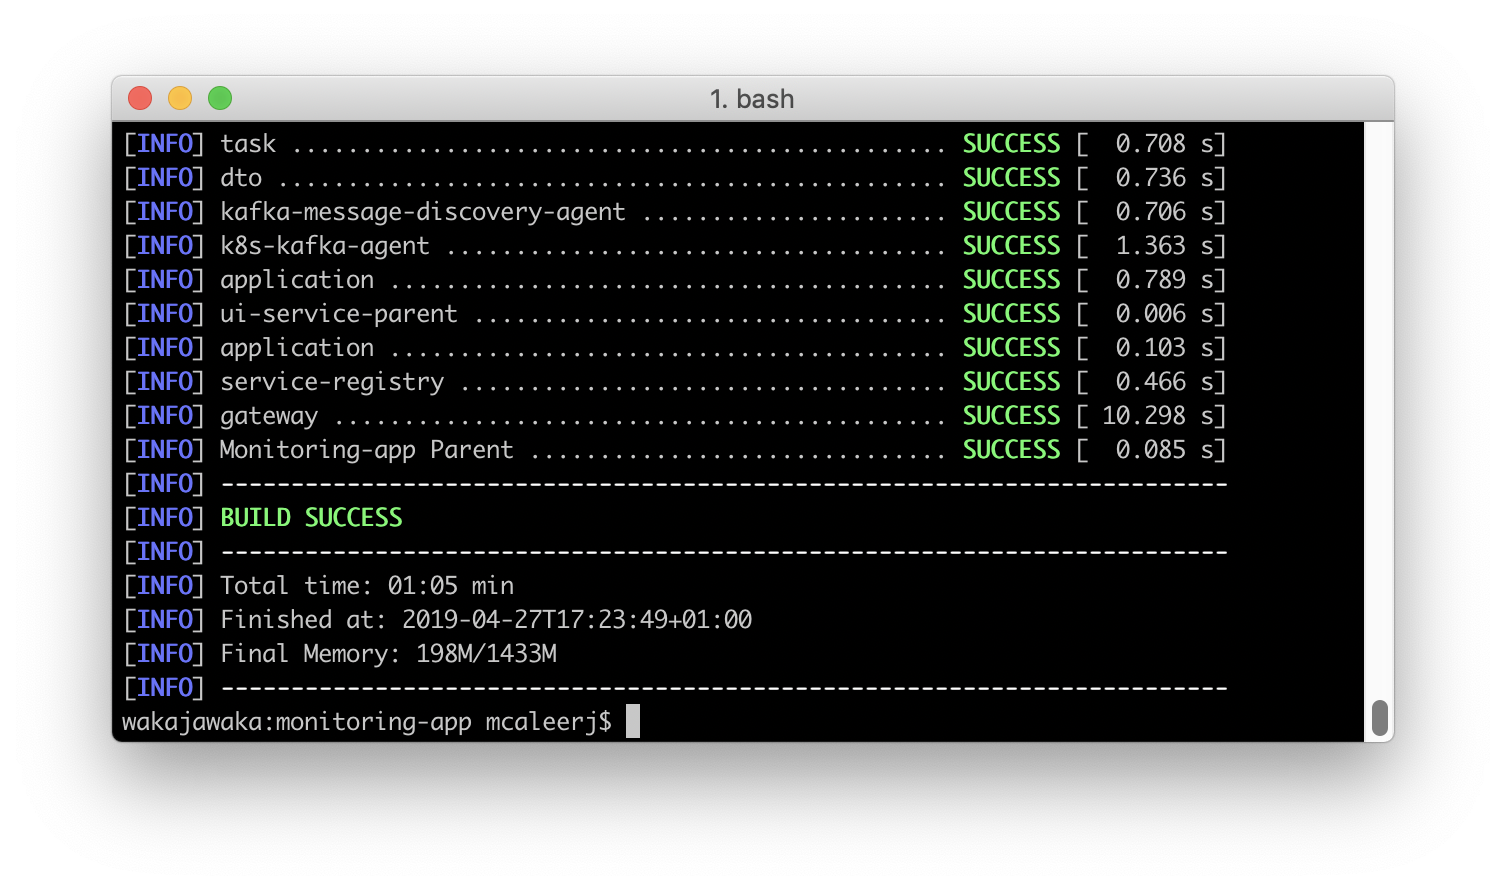
\includegraphics[width=\linewidth]{figures/appendixB/build-success.png}
	\caption{Successful build of Monitoring Application.}
	\label{monitoring_app_build_ok}
\end{figure}
\end{itemize}

\section{Running the Application}

To start each of the application microservices in turn, execute the following commands. It is recommend that each microservice run in a dedicated console for ease of log analysis.

\begin{enumerate}

	\item Start the Service Registry.
\begin{lstlisting}[language=bash]
cd service-registry
java -jar target/service-registry-0.0.1-SNAPSHOT.jar  
\end{lstlisting}	

	\item Start the Management Service.
\begin{lstlisting}[language=bash]
cd managementservice
java -jar application/target/management-service-application-0.0.1-SNAPSHOT.jar 
\end{lstlisting}	

	\item Start the Monitoring Service.
\begin{lstlisting}[language=bash]
cd monitorservice
java -jar application/target/monitoring-service-application-0.0.1-SNAPSHOT.jar
\end{lstlisting}	

	\item Start the Aggregation Service.
\begin{lstlisting}[language=bash]
cd aggregationservice
java -jar application/target/aggregation-service-application-0.0.1-SNAPSHOT.jar
\end{lstlisting}	

	\item Start the Discovery Service.
\begin{lstlisting}[language=bash]
cd discoveryservice
java -jar application/target/discovery-service-application-0.0.1-SNAPSHOT.jar
\end{lstlisting}	

	\item Start the Correlation Service.
\begin{lstlisting}[language=bash]
cd correlationservice
java -jar application/target/correlation-service-application-0.0.1-SNAPSHOT.jar
\end{lstlisting}	

	\item Start the UI Service.
\begin{lstlisting}[language=bash]
cd uiservice
java -jar application/target/ui-service-application-0.0.1-SNAPSHOT.jar
\end{lstlisting}	

	\item Start the Gateway Service.
\begin{lstlisting}[language=bash]
cd gatewayservice
java -jar target/gateway-service-0.0.1-SNAPSHOT.jar
\end{lstlisting}	

\end{enumerate}

Verify that all services are registered with the service registry by opening http://localhost:9091. A Eureka server user interface should list all seven microservices with status \texttt{UP}.
\begin{figure}[H]
	\centering  
	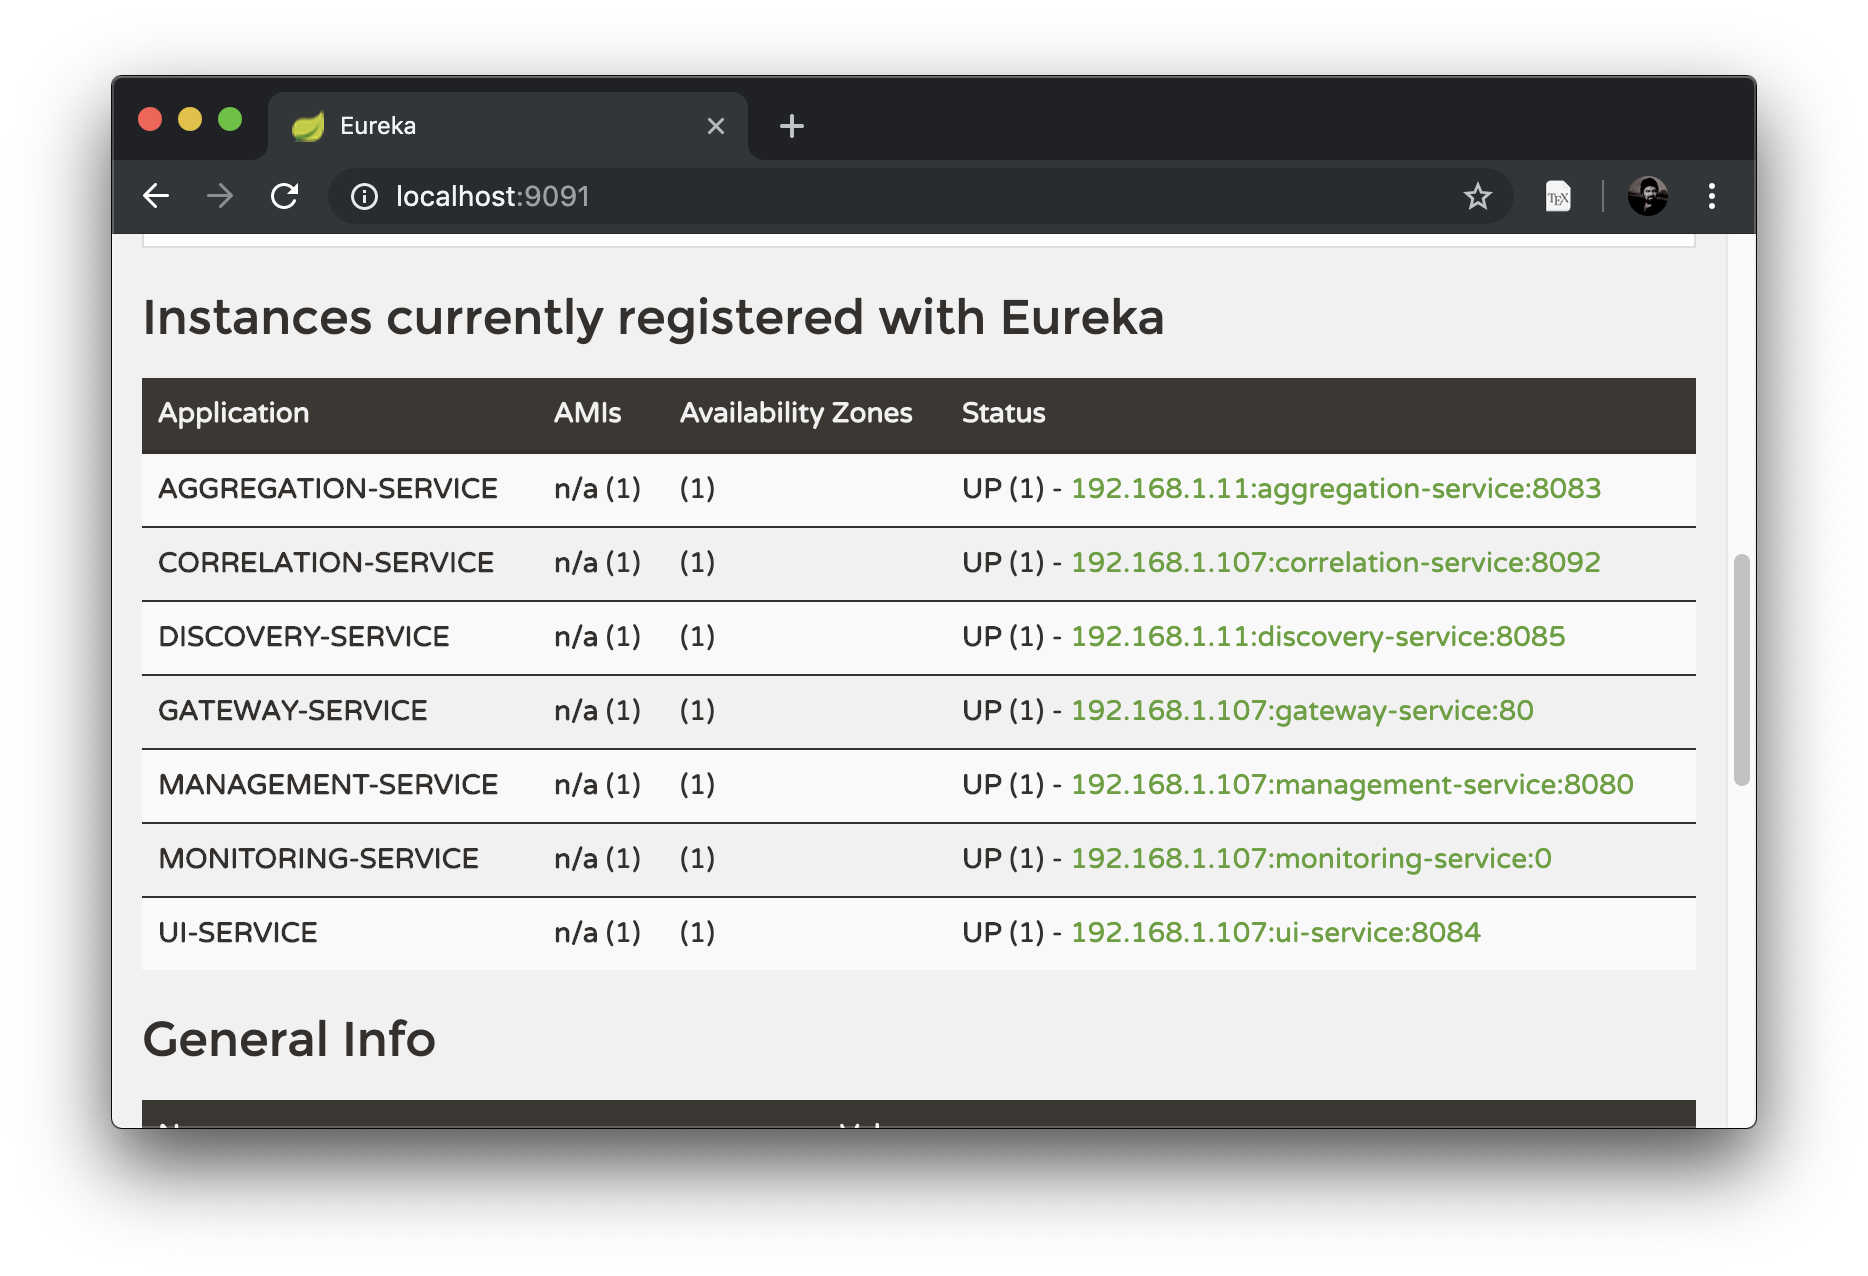
\includegraphics[width=\linewidth]{figures/appendixB/eureka.png}
	\caption{Service Registry UI lists all services as UP.}
\end{figure}